% Section content template for individual Educative lessons
% This file contains the actual content for a specific section
% Generated from Educative API section content

% Section: Evaluation of WhatsApp’s Design
% Section ID: 4861549654573056
% Section Slug: evaluation-of-whatsapps-design
% Generated: 2025-12-08T15:00:50.352282

\subsection{Requirements compliance}\label{6HUkOi81ULZId-hQclKsq}
\\
Our non-functional requirements for the proposed WhatsApp design are low latency, consistency, availability, and security. Let 's discuss how we have achieved these requirements in our system:

\begin{itemize}
\item
\protect\phantomsection\label{L4rHGQk10MuGpA6uJs0hy}
\textbf{Low latency}: We can minimize the latency of the system at various levels:

\begin{itemize}
\item
We can do this through geographically distributed WebSocket servers and the cache associated with them.
\item
We can use Redis cache clusters on top of MySQL database clusters.
\item
We can use CDNs for frequently sharing documents and media content.
\end{itemize}
\item
\protect\phantomsection\label{kPq9eh3g7Pc1gLH6nZpPG}
\textbf{Consistency}: The system also provides high consistency in messages with the help of a FIFO messaging queue with strict ordering. However, the ordering of messages would require the \href{https://www.educative.io/courses/grokking-the-system-design-interview/system-design-sequencer}{Sequencer} to provide ID with appropriate causality inference mechanisms to each message. For offline users, the Mnesia database stores messages in a queue. The messages are sent later in a sequence after the user goes online.
\item
\protect\phantomsection\label{S785WxJL5Wya0ISEUq3G4}
\textbf{Availability}: The system can be made highly available if we have enough WebSocket servers and replicate data across multiple servers. When a user gets disconnected due to some fault in the WebSocket server, the session is re-created via a load balancer with a different server. Moreover, the messages are stored on the Mnesia cluster following the primary-secondary replication model, which provides high availability and durability.
\item
\protect\phantomsection\label{XGWOXs9WeS6yY_4YrB7Jz}
\textbf{Security}: The system also provides an end-to-end encryption mechanism that secures the chat between users.
\item
\protect\phantomsection\label{tCXV-vFl6FC-JGGspk0J3}
\textbf{Scalability:} Due to high-performance engineering, scalability might not be a significant issue, as WhatsApp can handle around 10 million connections per server. However, our proposed system is flexible, as more servers can be added or removed as the load increases or decreases.
\end{itemize}

\begin{quote}
\textbf{Quiz:}
\textbf{Question 1:} In the event of a network partition, what should the system choose to compromise between consistency and availability?
\textbf{Answer:} According to the CAP theorem, the system would provide either consistency or availability in the event of a network partition. In our system of a WhatsApp messenger, the correct ordering of messages is essential. Otherwise, the context of the information communicated between users might change significantly. Therefore, availability in our system can take a hit if the network partition occurs.
\end{quote}

\textbf{Non-functional Requirements Compliance}

\begin{table}[htbp]
\centering
\small
\adjustbox{max width=\textwidth}{
\begin{tabular}{|p{0.246\textwidth}|p{0.704\textwidth}|}
\hline
\textbf{Non-functional Requirements} & \textbf{Approaches} \\
\hline
\hline
Minimizing latency & \begin{itemize} \tightlist \item Geographically distributed cache management systems and servers \item CDNs \end{itemize} \\
\hline
Consistency & \begin{itemize} \tightlist \item Provide unique IDs to messages using Sequencer or other mechanisms \item Use FIFO messaging queue with strict ordering \end{itemize} \\
\hline
Availability & \begin{itemize} \tightlist \item Provide multiple WebSocket servers and managers to establish connections between users \item Replication of messages and data associated with users and groups on different servers \item Follow disaster recovery protocols \end{itemize} \\
\hline
Security & \begin{itemize} \tightlist \item Via end-to-end encryption \end{itemize} \\
\hline
Scalability & \begin{itemize} \tightlist \item Performance tuning of servers \item Horizontal scalability of services \end{itemize} \\
\hline
\end{tabular}
}
\caption{Non-functional Requirements Compliance}
\end{table}

\subsection{Trade-offs}\label{ORCxt4Ofks1hYkAt-vSH8}
\\
We've seen that our proposed WhatsApp system fulfills the functional and non-functional requirements. However, two major trade-offs exist in the proposed WhatsApp design:

\begin{itemize}
\item
\protect\phantomsection\label{YXSWSEsWbr8PMkZRfKWfK}
There's a trade-off between consistency and availability.
\item
\protect\phantomsection\label{9MQzI4z71aDkb1pqkLHpq}
There's a trade-off between latency and security.
\end{itemize}

\subsubsection{The trade-off between consistency and availability}\label{YazSUPP2d8Z-s7rnCnvbU}
\\
According to the CAP theorem, in the event of a network failure or partition, the system can provide either consistency or availability. So , in the case of our WhatsApp design, we have to choose either consistency or availability. In
WhatsApp, the order of messages sent or received by a user is essential. Therefore, we should prioritize consistency rather than availability.

\subsubsection{The trade-off between latency and security}\label{zNABtu0z_P1OK6y4K74hv}
\\
Low latency is an essential factor in system design that provides a real-time experience to users. However, on the other side, sharing information or data over WhatsApp might be insecure without encryption. The absence of a proper security mechanism makes the data vulnerable to unauthorized access. So , we can accept a trade-off prioritizing the secure transmission of messages over low latency.
\\
\hfill\break
We might wonder where the trade-off is. Often, communication involves multimedia. Encrypting them in near real-time on the sender device and decrypting on the receiver side can be taxing for the devices, causing latency. The process is illustrated in the following figure:

\begin{figure}[htbp]
 \centering
 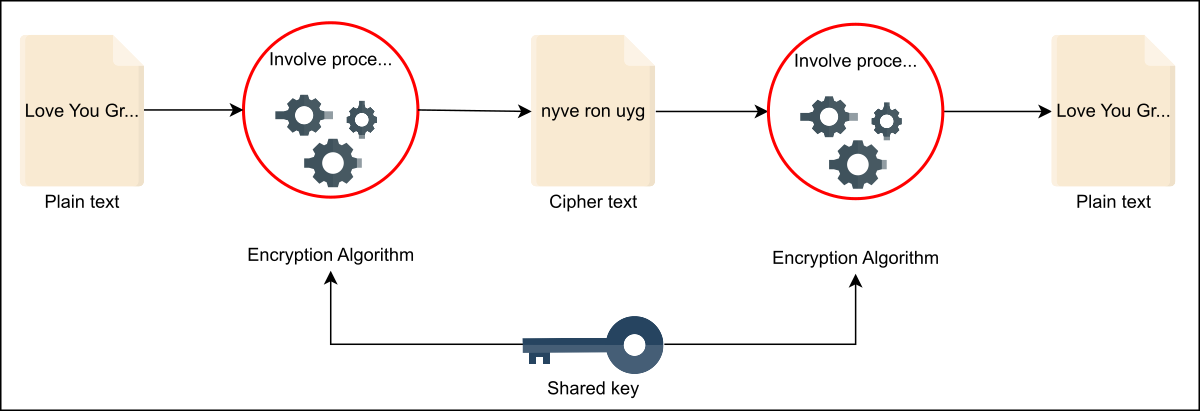
\includegraphics[width=0.5\textwidth]{Images/chapter_36/section_4861549654573056/4561363196444672.png}
 \caption{End-to-end encryption causes a delay in processing, which has an impact on latency}
\end{figure}

\subsection{Summary}\label{0Fnx_mu_ndungqGjQsTeM}
\\
In this chapter, we designed a WhatsApp messenger. First , we identified the functional and non-functional requirements along with the resources estimation crucial for the design. Second
, we focused on the high-level and detailed design of the WhatsApp system, where we described various components responsible for different services. Finally , we evaluated the non-functional requirements and highlighted some trade-offs in the design.\\
\strut \\
This design problem highlighted that we can optimize general-purpose computational resources for specific use cases. Whats App optimized its software stack to handle a substantially large number of connections on the commodity servers.

% End of section content